\headline{{\textbf{\Large\sffamily Bonsai Roots:}}\\
          {\textbf{\large\sffamily Meet the Members of TWBC}}}
\label{2025-09-roots}
\noindent
In every edition of \emph{Bonsai Roots,} we take a break from pruning and potting to spotlight the members who bring our club to life.
Each story adds a branch to the growing canopy of TWBC.
This month, we're delighted to introduce \textbf{Victoria Miquel}!

\begin{itemize}
    \item \textbf{What's your name and where in the country do you live?}

    \emph{My name is Victoria and I live in the West London area.}

    \item \textbf{What are your favourite species of tree and why?}

    \emph{Atlantic cedars --- they are very graceful! I also love maples for their colours, and flowering trees like plums and quinces.}

    \item \textbf{What aspect of bonsai do you enjoy?}

    \emph{It highlights the beauty of nature and makes you look forward to the future.}

    \item \textbf{What aspects of bonsai do you find most challenging?}

    \emph{Patience!}

    \begin{window}[%
        2,l,%
        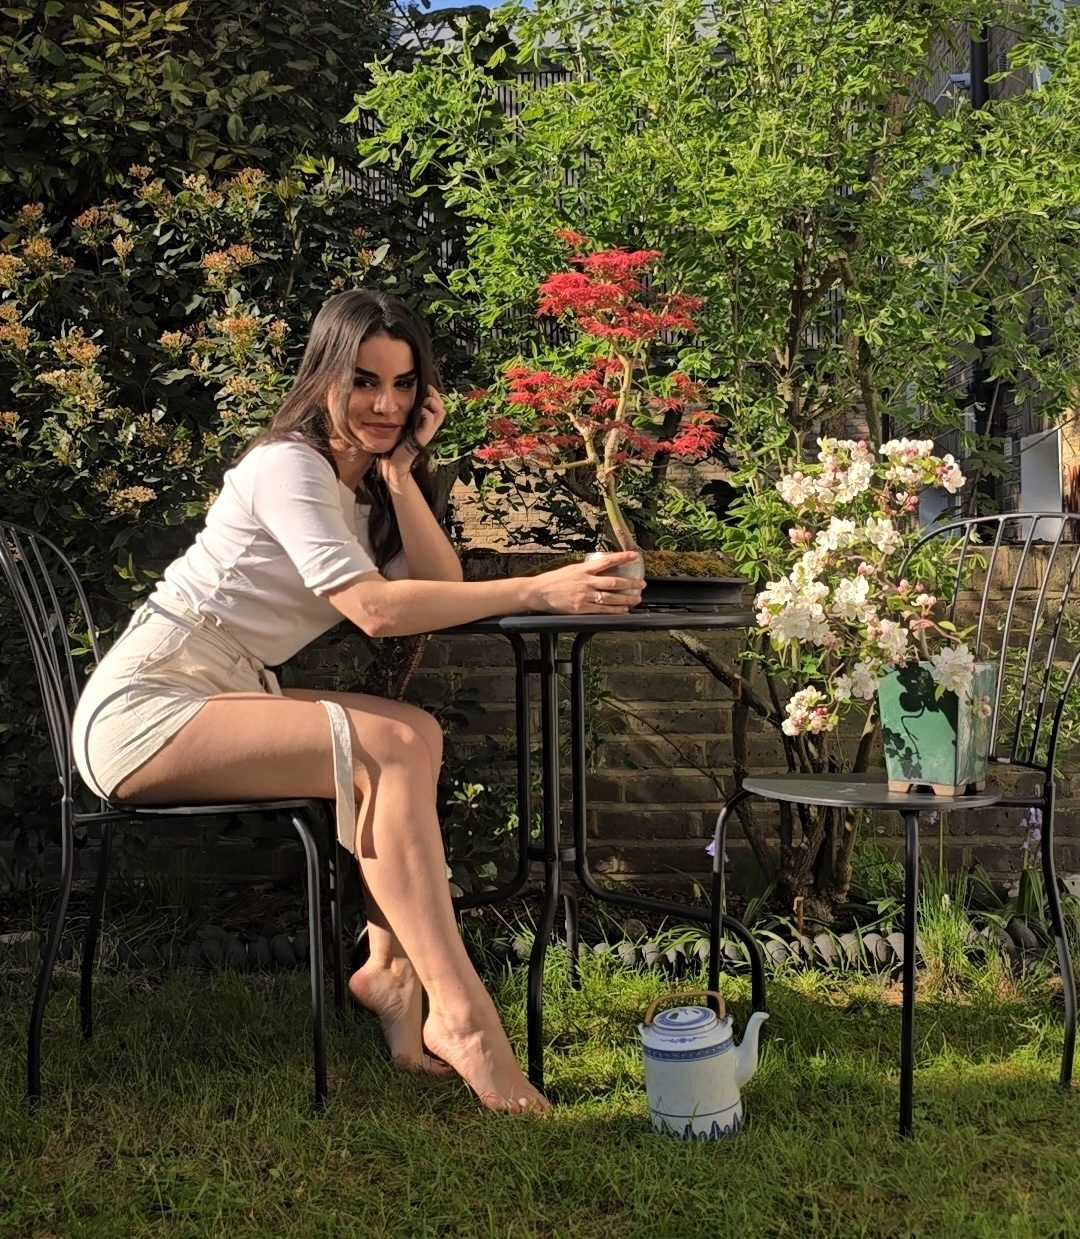
\includegraphics[width=1.0\columnwidth]{2025_09/res/roots_victoria},%
        \centerline{\emph{Victoria with a Japanese maple and a flowering quince.}}%
    ]
    \end{window}
    \columnbreak

    \item \textbf{Who or what inspires you throughout your bonsai journey?}

    \emph{Artists like \href{https://www.instagram.com/andbonsai}{Anrija Zokic} and \href{https://www.instagram.com/teppei_kojima501}{Teppei Kojima}, or those who first introduced me to bonsai: \href{https://www.youtube.com/@georgeomi2303}{Mr. Georges Omi}, whom I discovered on YouTube, and a friend from back home --- \href{https://beynes.fr/association/les\--amis\--du\--bonsai\--78}{Alain Tabary} --- who is becoming a recognised artist.}

    \item \textbf{How long have you been interested in keeping bonsai?}

    \emph{13 years.}

    \item \textbf{What stimulated your interest in bonsai?}

    \emph{I've always been into art and gardening --- bonsai sits at the intersection of both.}

    \item \textbf{If you could give someone new to bonsai any tips, what would it be?}

    \emph{Start with trees that grow fast and generate a lot of work --- it keeps you engaged and learning.}

    \item \textbf{Why do you enjoy being part of TWBC, and do you have any ideas or suggestions for the club's future?}

    \emph{I'm so happy to have found a club in London where I can continue my training and meet people who share this passion. I'd love to see monthly themes include seasonal trees --- like plums in February, azaleas in June, and maples in autumn.}

    \item \textbf{One word to describe what bonsai means to you?}

    \emph{Art.}

    \item \textbf{What are your future goals regarding your own trees and learning more about the hobby?}

    \emph{I want to grow old with my trees and bring them to exhibition level --- especially the first ones I worked on. I also hope to learn more about advanced methods of culture and shaping.}

    \item \textbf{How would you like to see your bonsai journey progress in the future?}

    \emph{My aim is to pass certification (at least level 1) and to help develop a more ``European'' aesthetic in bonsai, working with species and styles native to our region.}
\end{itemize}

Victoria's journey blends artistic vision with long\--term dedication --- and a deep appreciation for seasonal beauty.
Who will we meet next time?
Stay tuned for more in \emph{Bonsai Roots}!

\begin{center}
    $\cdots$
\end{center}

\noindent
\emph{If you're a newer member and would like to feature in a future edition of Bonsai Roots, simply fill out the form at \href{https://forms.gle/quVXa4L8rhpnT5kr6}{this link}! We'd love to hear your story.}

\closearticle
\columnbreak
